\documentclass[aspectratio=169]{beamer}
\usetheme{Madrid}
\usecolortheme{beaver}

% Packages
\usepackage{amsmath,amssymb,amsthm}
\usepackage{algorithm}
\usepackage{algpseudocode}
\usepackage{tikz}
\usepackage{pgfplots}
\usepackage{booktabs}
\usepackage{multirow}
\usepackage{graphicx}
\usepackage{xcolor}
\usepackage{hyperref}
% Prevent translator/hyperref interaction warnings in PDF strings
\pdfstringdefDisableCommands{\def\translate#1{#1}}
\usepackage{pifont} % provides \ding for checkmarks and dingbats

% Beamer/amsthm provide theorem-like environments; avoid redefinition here.
\pgfplotsset{compat=1.18}
\usetikzlibrary{graphs,arrows.meta,positioning,shapes}

% Custom colors
\definecolor{darkred}{RGB}{139,0,0}
\definecolor{darkgreen}{RGB}{0,100,0}
\definecolor{darkblue}{RGB}{0,0,139}

% Title page information
\title[Feedback Vertex Set]{The Feedback Vertex Set Problem:\\Theory, Algorithms, and Applications}
\subtitle{Project Checkpoint Presentation, CSE 462}
\author[Group-06]{2005090 - Tawkir Aziz Rahman \\
		2005074 - Dipanta Kumar Roy Nobo \\
		2005091 - Waseem Mustak Zisan \\
		2005104 - Hasin Arafat \\
		2005109 - Noushin Tabassum Aoishy \\
		2005068 - Suman Hossain}
\institute[CSE,BUET]{Department of Computer Science and Engineering, Bangladesh University of Engineering and Technology}
\date{\today}

% Custom commands
\newcommand{\fvs}{\textsc{FVS}}
\newcommand{\np}{\textsc{NP}}
\newcommand{\opt}{\textsc{OPT}}

\begin{document}

% Title slide
\begin{frame}
	\titlepage
\end{frame}

% Table of contents
\begin{frame}{Outline}
	\tableofcontents
\end{frame}


% ============================================
% SECTION 1: PROBLEM DEFINITION
% ============================================
\section{Problem Definition}

\begin{frame}{Problem Definition}
	\begin{block}{Overview}
		\begin{itemize}
			\item Define the Feedback Vertex Set (\fvs) problem and formal statement.
			\item Provide visual examples and intuition (cycles vs. forests).
			\item Highlight key properties: NP-completeness and FPT results.
		\end{itemize}
	\end{block}
\end{frame}

\begin{frame}{What is the Feedback Vertex Set Problem?}
	\begin{definition}[Feedback Vertex Set]
		Given an undirected graph $G = (V, E)$ and an integer $k$, find a set $S \subseteq V$ with $|S| \leq k$ such that $G - S$ is \textbf{acyclic} (a forest).
	\end{definition}

	\vspace{0.3cm}

	\begin{columns}[T]
		\column{0.5\textwidth}
		\textbf{Formal Problem:}
		\begin{itemize}
			\item \textbf{Input:} Graph $G = (V,E)$, integer $k$
			\item \textbf{Question:} $\exists S \subseteq V$, $|S| \leq k$ such that $G-S$ has no cycles?
			\item \textbf{Optimization:} Find minimum $|S|$
		\end{itemize}

		\column{0.5\textwidth}
		\textbf{Intuition:}
		\begin{itemize}
			\item Break all cycles by removing vertices
			\item Every cycle must contain $\geq 1$ vertex from $S$
			\item Minimize disruption (minimize $|S|$)
		\end{itemize}
	\end{columns}
\end{frame}

\begin{frame}{Visual Examples}
	\begin{columns}[T]<1->
		\column{0.33\textwidth}
		\centering
		\textbf{Triangle (3-cycle)}\\[0.2cm]
		\begin{tikzpicture}[scale=0.8]
			\only <1>{\node[circle,draw, fill=red!30] (1) at (0,1.5) {1};}
            \only <2->{\node (1) at (0,1.5) {};}
			\node[circle,draw] (2) at (-1,0) {2};
			\node[circle,draw] (3) at (1,0) {3};
			\only <1>{\draw[thick] (1) -- (2) -- (3) -- (1);}
			\only<2-> {\draw[thick] (2) -- (3);}
		\end{tikzpicture}\\[0.1cm]
		\only <2->{\small \fvs = \{1\}, Size = 1}

		\column{0.33\textwidth}
		\centering
		\textbf{Complete Graph $K_4$}\\[0.2cm]
		\begin{tikzpicture}[scale=0.8]
			\only<1-2> {\node[circle,draw] (1) at (0,1.5) {1};}
			\only<3> {\node[circle,draw,fill=red!30] (1) at (0,1.5) {1};}
			\only<4-> {\node (1) at (0,1.5) {};}
			\only<1-3> {\node[circle,draw] (2) at (-1,0) {2};}
			\only<4>{\node[circle,draw,fill=red!30] (2) at (-1,0) {2};}
			\only<5->{\node (2) at (-1,0) {};}
			\node[circle,draw] (3) at (1,0) {3};
			\node[circle,draw] (4) at (0,-0.5) {4};
			\only <1-3>{\draw[thick] (1) -- (2) -- (3) -- (4) -- (1);}
			\only <4-> {\draw[thick] (3) -- (4);} 
			\only <4> {\draw[thick] (2) -- (3);} 
			\only <1-3>{\draw[thick] (1) -- (3);}
			\only <1-4>{\draw[thick] (2) -- (4);}
		\end{tikzpicture}\\[0.1cm]
		\only <5-> {\small \fvs = \{1,2\}, Size = 2}

		\column{0.33\textwidth}
		\centering
		\textbf{Tree}\\[0.2cm]
		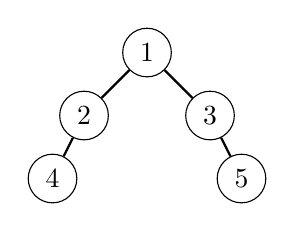
\begin{tikzpicture}[scale=0.8]
			\node[circle,draw] (1) at (0,1.5) {1};
			\node[circle,draw] (2) at (-1,0.5) {2};
			\node[circle,draw] (3) at (1,0.5) {3};
			\node[circle,draw] (4) at (-1.5,-0.5) {4};
			\node[circle,draw] (5) at (1.5,-0.5) {5};
			\draw[thick] (1) -- (2);
			\draw[thick] (1) -- (3);
			\draw[thick] (2) -- (4);
			\draw[thick] (3) -- (5);
		\end{tikzpicture}\\[0.1cm]
		\only<7->{\small \fvs = $\emptyset$, Size = 0}
	\end{columns}

	\vspace{0.5cm}
	\begin{alertblock}{Key Property}
		A set $S$ is a feedback vertex set if and only if removing $S$ leaves no cycles.
	\end{alertblock}
\end{frame}


\begin{frame}{Important Properties}
\begin{enumerate}
	\item<1-> \textbf{NP-Completeness:} \fvs\ is \np-complete (shown via reductions from problems such as Vertex Cover).\\
				\small A problem is NP-complete if it is in NP and every problem in NP can be reduced to it in polynomial time.

	\item<2-> \textbf{Parameterized Complexity:} Fixed-Parameter Tractable (FPT).
				\begin{itemize}
					\item<3-> Solvable in $O(f(k)\cdot\mathrm{poly}(n))$ time.
					\item<3-> One of the best known FPT algorithms runs in time $O(c^k\cdot\mathrm{poly}(n))$ for some $c<4$.
				\end{itemize}

	\item<4-> \textbf{Bounds:}
				\begin{itemize}
					\item<4-> A commonly used heuristic lower bound is $|E| - |V| + c$ (where $c$ = number of connected components).
					\item<4-> Upper bound example: $|S| \leq |V| - 1$.
				\end{itemize}

	\item<5-> \textbf{Special Cases:}
				\begin{itemize}
					\item<5-> Trees/Forests: $|S| = 0$.
					\item<5-> Planar graphs: Better approximation algorithms exist.
				\end{itemize}
\end{enumerate}
\end{frame}





% ============================================
% SECTION 2: REDUCTIONS
% ============================================


\section{Polynomial-Time Reductions}

\begin{frame}{Reductions: Why They Matter}
  \begin{block}{Purpose of Reductions}
    \begin{itemize}
      \item Prove \fvs\ is \np-hard by reducing from known \np-complete problems
      \item Show relationships between different hard problems
      \item Transfer algorithmic techniques between problem domains
    \end{itemize}
  \end{block}
  
  \vspace{0.5cm}
  
  \begin{columns}[T]
    \column{0.5\textwidth}
    \textbf{Key Reductions:}
		\begin{itemize}
			\item \textcolor{blue}{Vertex Cover $\rightarrow$ \fvs}
			\item \textcolor{blue}{\fvs $\rightarrow$ Vertex Cover}
			\item 3-SAT $\rightarrow$ \fvs
			\item \fvs $\rightarrow$ Independent Set problem
		\end{itemize}
    
    \column{0.5\textwidth}
    \textbf{Complexity Implications:}
    \begin{itemize}
      \item \fvs\ is \np-complete
      \item No polynomial algorithm unless P=NP
      \item Same approximation barriers as Vertex Cover
    \end{itemize}
  \end{columns}
\end{frame}

\begin{frame}{Reduction 1: Vertex Cover $\rightarrow$ \fvs}
  \begin{block}{Vertex Cover (VC) Problem}
    Find smallest $S \subseteq V$ such that every edge has at least one endpoint in $S$.
  \end{block}
  
  \vspace{0.3cm}
  
  \textbf{Construction:} Given VC instance $(G,k)$
  \begin{enumerate}
    \item For each edge $e = (u,v) \in E(G)$:
    \begin{itemize}
      \item Add new vertex $w_e$
      \item Form triangle: edges $(u,v)$, $(u,w_e)$, $(v,w_e)$
    \end{itemize}
    \item Keep same parameter $k' = k$
  \end{enumerate}
  
  \vspace{0.3cm}
  
  \begin{theorem}
    $G$ has VC of size $\leq k$ $\Leftrightarrow$ $G'$ has \fvs\ of size $\leq k$
  \end{theorem}
  
  \textbf{Time:} $O(|E|)$ (polynomial)
\end{frame}

\begin{frame}{VC $\rightarrow$ \fvs: Example \& Proof}
  \begin{columns}[T]
    \column{0.45\textwidth}
    \textbf{Original Graph $G$:}
    \begin{center}
    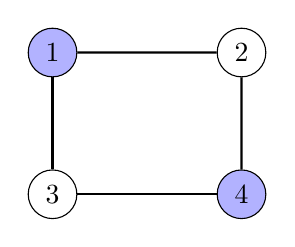
\begin{tikzpicture}[scale=1.2]
      \node[circle,draw,fill=blue!30] (1) at (0,1.5) {1};
      \node[circle,draw] (2) at (2,1.5) {2};
      \node[circle,draw] (3) at (0,0) {3};
      \node[circle,draw,fill=blue!30] (4) at (2,0) {4};
      \draw[thick] (1) -- (2);
      \draw[thick] (2) -- (4);
      \draw[thick] (4) -- (3);
      \draw[thick] (3) -- (1);
    \end{tikzpicture}
    \end{center}
    \small
    Minimum Vertex Cover: $\{1,4\}$ (size=2)\\
    Covers edges: (1,2), (2,4), (4,3), (3,1)
    
    \column{0.55\textwidth}
    \textbf{Transformed Graph $G'$:}
    \begin{center}
    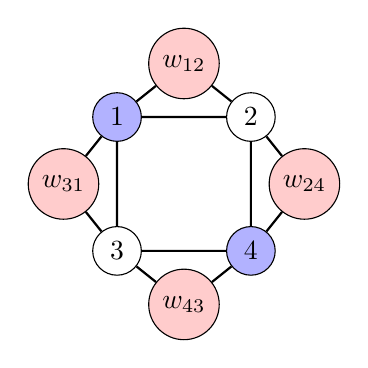
\begin{tikzpicture}[scale=0.85]
      \node[circle,draw,fill=blue!30] (1) at (0,2) {1};
      \node[circle,draw] (2) at (2,2) {2};
      \node[circle,draw] (3) at (0,0) {3};
      \node[circle,draw,fill=blue!30] (4) at (2,0) {4};
      \node[circle,draw,fill=red!20] (w12) at (1,2.8) {$w_{12}$};
      \node[circle,draw,fill=red!20] (w24) at (2.8,1) {$w_{24}$};
      \node[circle,draw,fill=red!20] (w43) at (1,-0.8) {$w_{43}$};
      \node[circle,draw,fill=red!20] (w31) at (-0.8,1) {$w_{31}$};

\draw[thick] (1) -- (2) -- (w12) -- (1);  % Triangle for edge 1-2
      \draw[thick] (2) -- (4) -- (w24) -- (2);  % Triangle for edge 2-4
      \draw[thick] (4) -- (3) -- (w43) -- (4);  % Triangle for edge 4-3
      \draw[thick] (3) -- (1) -- (w31) -- (3);  % Triangle for edge 3-1
    \end{tikzpicture}
    \end{center}
    \small
    \fvs: $\{1,4\}$ breaks all 4 triangles\\
    Each triangle = one original edge
  \end{columns}
  
  \vspace{0.3cm}
	% \begin{proof}[Proof Sketch]
	%   \begin{itemize}
	%     \item $\Rightarrow$: VC hits each original edge $\rightarrow$ removes one vertex from each triangle $\rightarrow$ breaks all cycles
	%     \item $\Leftarrow$: \fvs\ must contain $\ge 1$ vertex from each triangle $\rightarrow$ corresponds to VC in original graph
	%   \end{itemize}
	% \end{proof}
\end{frame}

\begin{frame}{Reduction 2: \fvs $\rightarrow$ Vertex Cover}
  \begin{block}{Reverse Direction}
    Shows Vertex Cover and \fvs\ are polynomially equivalent
  \end{block}
  
  \vspace{0.3cm}
  
  \textbf{Construction:} Given \fvs\ instance $(G,k)$
  \begin{enumerate}
    \item Replace each vertex $v \in V$ with triangle $\{v_1, v_2, v_3\}$
    \item For each edge $(u,v) \in E$, connect triangles with cross edges
    \item Set $k' = 2|V| + k$
  \end{enumerate}
  
  \vspace{0.3cm}
  
  \begin{theorem}
    $G$ has \fvs\ of size $\leq k$ $\Leftrightarrow$ $G'$ has VC of size $\leq 2|V| + k$
  \end{theorem}
  
  \textbf{Key Insight:} 
  \begin{itemize}
	\item Each triangle needs $\ge 2$ vertices in VC
	\item Triangles with 3 vertices in VC $\leftrightarrow$ vertices in \fvs
  \end{itemize}
\end{frame}

\begin{frame}{\fvs $\rightarrow$ VC: Visual Example}
  \begin{columns}[T]
    \column{0.4\textwidth}
    \textbf{Original Graph $G$:}
    \begin{center}
    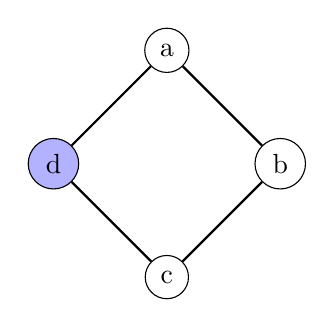
\begin{tikzpicture}[scale=1.2]
      \node[circle,draw] (a) at (90:1.2) {a};
      \node[circle,draw] (b) at (0:1.2) {b};
      \node[circle,draw] (c) at (270:1.2) {c};
      \node[circle,draw,fill=blue!30] (d) at (180:1.2) {d};
      \draw[thick] (a) -- (b) -- (c) -- (d) -- (a);
    \end{tikzpicture}
    \end{center}
    \small
    \fvs: $\{d\}$ (size=1)\\
    Removing $d$ breaks the 4-cycle
    
    \column{0.6\textwidth}
    \textbf{Transformed Graph $G'$ (simplified view):}
    \begin{center}
    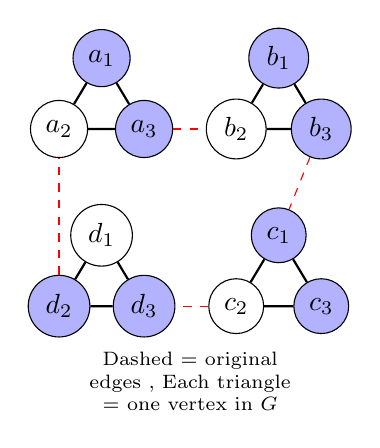
\begin{tikzpicture}[scale=0.9]
      % Triangles spaced out
      \node[circle,draw,fill=blue!30] (a1) at (0,2.5) {$a_1$};
      \node[circle,draw] (a2) at (-0.6,1.5) {$a_2$};
      \node[circle,draw,fill=blue!30] (a3) at (0.6,1.5) {$a_3$};
      \draw[thick] (a1) -- (a2) -- (a3) -- (a1);
      
      \node[circle,draw,fill=blue!30] (b1) at (2.5,2.5) {$b_1$};
      \node[circle,draw] (b2) at (1.9,1.5) {$b_2$};
      \node[circle,draw,fill=blue!30] (b3) at (3.1,1.5) {$b_3$};
      \draw[thick] (b1) -- (b2) -- (b3) -- (b1);
      
      \node[circle,draw] (d1) at (0,0) {$d_1$};
      \node[circle,draw,fill=blue!30] (d2) at (-0.6,-1) {$d_2$};
      \node[circle,draw,fill=blue!30] (d3) at (0.6,-1) {$d_3$};
      \draw[thick] (d1) -- (d2) -- (d3) -- (d1);
      
      \node[circle,draw,fill=blue!30] (c1) at (2.5,0) {$c_1$};
      \node[circle,draw] (c2) at (1.9,-1) {$c_2$};
      \node[circle,draw,fill=blue!30] (c3) at (3.1,-1) {$c_3$};
      \draw[thick] (c1) -- (c2) -- (c3) -- (c1);
      
      % Representative cross edges (just show pattern)
      \draw[dashed,red] (a3) -- (b2);
      \draw[dashed,red] (b3) -- (c1);
      \draw[dashed,red] (c2) -- (d3);
      \draw[dashed,red] (d2) -- (a2);
      
      \node[text width=3cm,align=center,font=\scriptsize] at (1.25,-2) {\\Dashed = original edges , Each triangle = one vertex in $G$};
    \end{tikzpicture}
    \end{center}
  \end{columns}
  
  \vspace{0.3cm}
	\begin{minipage}{\textwidth}
		\small
		\textbf{Vertex Cover in $G'$: is also a FVS}
	\begin{itemize}
		\item Each triangle needs $\ge 2$ vertices in VC
		\item Triangles with 3 vertices in VC $\leftrightarrow$ vertices in \fvs
	\end{itemize}
	\end{minipage}
\end{frame}

\begin{frame}{Other Important Reductions}
	\begin{block}{3-SAT $\rightarrow$ \fvs (Standard NP-hardness proof)}
    \begin{itemize}
      \item \textbf{Variable gadget:} Triangle $\{x, \neg x, t_x\}$
      \item \textbf{Clause gadget:} Cycle connecting 3 literal vertices
	\item \textbf{Reduction:} $\phi$ satisfiable $\leftrightarrow$ $G_\phi$ has \fvs\ of size $n$
      \item \textbf{Time:} $O(n+m)$ (linear)
    \end{itemize}
  \end{block}
  
  \vspace{0.5cm}
  
  \begin{block}{Quick Examples of Other Reductions}
    \begin{itemize}
	% \item \textbf{\fvs $\rightarrow$ Odd Cycle Transversal:} Subdivide edges, preserve parity
	\item \textbf{Independent Set $\rightarrow$ \fvs:} Via complement graph transformation
	\item \textbf{Dominating Set $\rightarrow$ \fvs:} On directed line graphs
    \end{itemize}
  \end{block}
\end{frame}

\begin{frame}{Reduction Complexity Summary}
  \begin{table}
    \centering
    \small
    \begin{tabular}{@{}lll@{}}
      \toprule
      \textbf{Reduction} & \textbf{Time} & \textbf{Preserves Solution Size?} \\
      \midrule
	Vertex Cover $\rightarrow$ \fvs & $O(|E|)$ & Yes (exactly) \\
	\fvs $\rightarrow$ Vertex Cover & $O(|V|+|E|)$ & Linear: $k' = 2|V| + k$ \\
	3-SAT $\rightarrow$ \fvs & $O(n+m)$ & Linear: $k' = n$ (\#variables) \\
	\fvs $\rightarrow$ Independent Set & $O(|V|+|E|)$ & Within factor 2 \\
      \bottomrule
    \end{tabular}
  \end{table}
  
  \vspace{0.8cm}
  
  \begin{block}{Key Takeaways}
    \begin{enumerate}
      \item Vertex Cover and \fvs\ are \textbf{polynomially equivalent}
      \item Both are \np-complete (reducible from 3-SAT)
      \item Reductions preserve approximation hardness
      \item Algorithmic techniques transfer between problems
    \end{enumerate}
  \end{block}
\end{frame}

\begin{frame}{Implications for Algorithms}
  \begin{columns}[T]
    \column{0.5\textwidth}
    \textbf{What We Gain:}
    \begin{itemize}
      \item \fvs\ inherits Vertex Cover's:
      \begin{itemize}
        \item 2-approximation algorithm
        \item Kernelization results
        \item FPT algorithms (parameter $k$)
        \item Branching techniques
      \end{itemize}
      \item Can use SAT solvers via 3-SAT reduction
    \end{itemize}
    
    \column{0.5\textwidth}
    \textbf{Limitations:}
    \begin{itemize}
      \item No polynomial algorithm (unless P=NP)
      \item Hard to approximate better than 2 (under UGC)
      \item W[1]-hard for some parameters
    \end{itemize}
  \end{columns}
  
  \vspace{0.8cm}
  
	\begin{alertblock}{The Big Picture}
		Reductions create a network of equivalent hard problems. Solving one efficiently would solve them all (unlikely under $\mathrm{P} \neq \mathrm{NP}$).
	\end{alertblock}
\end{frame}





\section{Existing Algorithms Survey}


\begin{frame}{Algorithm Survey}
	\begin{block}{Overview}
		\begin{itemize}
			\item Classify algorithms: Exact, Approximation, Randomized, Heuristic, Metaheuristic.
			\item Present representative methods and their time/quality trade-offs.
			\item Highlight algorithms selected for implementation and evaluation.
		\end{itemize}
	\end{block}
\end{frame}

% ============================================
% NEW COMPREHENSIVE ALGORITHM SLIDES
% ============================================

\begin{frame}{Five Major Categories of Solution Approaches}
    \small
    \begin{columns}[T]
        % Column 1: Exact + Approximation
        \column{0.25\textwidth}
        \begin{block}{1. Exact Exponential}
            \scriptsize
            \begin{itemize}
                \item Naive Brute Force
                \item DP on Subsets
                \item Iterative Compression
                \item Bounded Search Tree
                \item Current Best FPT
                \item Inclusion-Exclusion DP
            \end{itemize}
        \end{block}
        
        
        \begin{block}{2. Approximation}
            \scriptsize
            \begin{itemize}
                \item 2-Approximation (VC-based)
                \item Log-Approximation
                \item LP Rounding
                \item Primal-Dual
                \item Local Ratio
            \end{itemize}
        \end{block}
        
        % Column 2: Randomized + Heuristic
        \column{0.25\textwidth}
        \begin{block}{3. Randomized}
            \scriptsize
            \begin{itemize}
                \item Random Sampling
                \item Randomized Rounding
                \item Color Coding
            \end{itemize}
        \end{block}
        
        
        \begin{block}{4. Heuristic}
            \scriptsize
            \begin{itemize}
                \item Greedy Vertex Selection
                \item Cycle-Based Greedy
                \item Maximum Degree Heuristic
                \item Core-Periphery Decomposition
                \item Reduction Rules + Greedy
            \end{itemize}
        \end{block}
        
        % Column 3: Metaheuristic
        \column{0.25\textwidth}
        \begin{block}{5. Metaheuristic}
            \scriptsize
            \begin{itemize}
                \item Genetic Algorithm
                \item Simulated Annealing
                \item Ant Colony Optimization
                \item Tabu Search
                \item Particle Swarm Optimization
            \end{itemize}
        \end{block}
        
        % Optional: Add a placeholder or spacing to balance the column
        \vspace{1.8cm} % Adjust to match other columns visually
    \end{columns}
    
    \centering
    \vspace{0.2cm}
    \textbf{Total: 24+ algorithms surveyed across all categories}
\end{frame}
% ============================================
% Category 1: Exact Exponential Algorithms
% ============================================

\begin{frame}{Category 1: Exact Exponential Algorithms}
	\begin{table}
		\tiny
		\begin{tabular}{@{}p{3.2cm}p{5cm}p{2.5cm}p{2cm}@{}}
			\toprule
			\textbf{Algorithm}                                                                                           & \textbf{Description} & \textbf{Complexity} & \textbf{Solution Quality} \\
			\midrule

			\textbf{Naive Brute Force}                                                                                   &
			Enumerate all $2^n$ subsets and check if each forms a valid FVS using cycle detection                        &
			$O(2^n \cdot n^3)$                                                                                           &
			Optimal                                                                                                                                                                               \\
			\midrule

			\textbf{DP on Subsets}                                                                                       &
			Dynamic programming to avoid recomputing subproblems; for each subset, determine if it's a valid FVS         &
			$O(2^n \cdot n^2)$                                                                                           &
			Optimal                                                                                                                                                                               \\
			\midrule

			\textbf{Iterative Compression}                                                                               &
			FPT algorithm that assumes solution of size $k+1$ and compresses to size $k$ (Dehne et al., 2004)            &
			$O(5^k \cdot kn^2)$                                                                                          &
			Optimal                                                                                                                                                                               \\
			\midrule

			\textbf{Bounded Search Tree}                                                                                 &
			Use branching rules to create search tree with depth $\leq k$; improved branching factor (Chen et al., 2006) &
			$O(4^k \cdot n^2)$                                                                                           &
			Optimal                                                                                                                                                                               \\
			\midrule

			\textbf{Current Best FPT}                                                                                    &
			State-of-art using crown decomposition, sunflower lemma, refined branching (Kociumaka \& Pilipczuk, 2010)    &
			$O(3.619^k \cdot n^4)$                                                                                       &
			Optimal                                                                                                                                                                               \\
			\midrule

			\textbf{Inclusion-Exclusion DP}                                                                              &
			Uses inclusion-exclusion principle with DP for counting; fast for very small graphs ($n \leq 25$)            &
			$O(2^n \cdot n)$                                                                                             &
			Optimal                                                                                                                                                                               \\

			\bottomrule
		\end{tabular}
	\end{table}

	\vspace{0.2cm}
	\footnotesize
	\textbf{Key Insight:} FPT algorithms practical for $k \leq 50$; exponential in $n$ feasible only for $n \leq 20$
\end{frame}

% ============================================
% Category 2: Approximation Algorithms
% ============================================

\begin{frame}{Category 2: Approximation Algorithms}
	\begin{table}
		\tiny
		\begin{tabular}{@{}p{3.5cm}p{5.5cm}p{2cm}p{1.8cm}@{}}
			\toprule
			\textbf{Algorithm}                                                                                             & \textbf{Description} & \textbf{Complexity} & \textbf{Solution Quality} \\
			\midrule

			\textbf{2-Approximation (VC-based)}                                                                            &
			Reduce FVS to Vertex Cover; iteratively find cycles and remove both endpoints of any edge (Bafna et al., 1999) &
			$O(n^2)$                                                                                                       &
			2-approx                                                                                                                                                                                \\
			\midrule

			\textbf{Log-Approximation}                                                                                     &
			For tournament graphs using hitting set techniques; specific to directed complete graphs                       &
			$O(n^2 \log n)$                                                                                                &
			$O(\log n)$-approx                                                                                                                                                                      \\
			\midrule

			\textbf{LP Rounding}                                                                                           &
			Formulate as ILP, solve LP relaxation, then round fractional solution (deterministic or randomized)            &
			$O(n^{3.5})$                                                                                                   &
			2-approx                                                                                                                                                                                \\
			\midrule

			\textbf{Primal-Dual}                                                                                           &
			Maintain primal and dual solutions simultaneously; combinatorial approach without LP solver                    &
			$O(n^2)$                                                                                                       &
			2-approx                                                                                                                                                                                \\
			\midrule

			\textbf{Local Ratio}                                                                                           &
			Decompose weight function and apply local decisions; works well with weighted vertices                         &
			$O(n^2)$                                                                                                       &
			2-approx                                                                                                                                                                                \\

			\bottomrule
		\end{tabular}
	\end{table}

	\vspace{0.2cm}
	\footnotesize
	\textbf{Open Question:} Does $(2-\varepsilon)$-approximation exist? Under UGC, 2 might be optimal.
\end{frame}

% ============================================
% Category 3: Randomized Algorithms
% ============================================

\begin{frame}{Category 3: Randomized Algorithms}
	\begin{table}
		\tiny
		\begin{tabular}{@{}p{3.5cm}p{6cm}p{2cm}p{1.8cm}@{}}
			\toprule
			\textbf{Algorithm}                                                                                     & \textbf{Description} & \textbf{Complexity} & \textbf{Solution Quality} \\
			\midrule

			\textbf{Random Sampling}                                                                               &
			Randomly sample vertices in random order; if vertex in cycle, include it in FVS; Monte Carlo approach  &
			$O(n^2)$ per trial                                                                                     &
			Expected $O(\log n)$-approx                                                                                                                                                     \\
			\midrule

			\textbf{Randomized Rounding}                                                                           &
			Solve LP relaxation, then randomly include vertex $v$ with probability $x_v^*$; LP-based randomization &
			$O(n^3)$                                                                                               &
			Expected 2-approx                                                                                                                                                               \\
			\midrule

			\textbf{Color Coding}                                                                                  &
			Randomly color vertices and use DP to find colorful solutions; for bounded treewidth graphs            &
			$O(2^{O(k)} \cdot n)$                                                                                  &
			Optimal w.h.p.                                                                                                                                                                  \\

			\bottomrule
		\end{tabular}
	\end{table}

	\vspace{0.3cm}
	\footnotesize
	\begin{block}{Key Advantages}
		\begin{itemize}
			\item Probabilistic guarantees with high probability (w.h.p.)
			\item Can be derandomized using method of conditional expectations
			\item Excellent for sparse graphs and bounded treewidth structures
		\end{itemize}
	\end{block}
\end{frame}

% ============================================
% Category 4: Heuristic Algorithms
% ============================================

\begin{frame}{Category 4: Heuristic Algorithms}
	\begin{table}
		\tiny
		\begin{tabular}{@{}p{3.5cm}p{5.5cm}p{2cm}p{2cm}@{}}
			\toprule
			\textbf{Algorithm}                                                                          & \textbf{Description} & \textbf{Complexity} & \textbf{Solution Quality} \\
			\midrule

			\textbf{Greedy Vertex Selection}                                                            &
			Repeatedly remove vertex with maximum degree; simple and fast; uses priority queue          &
			$O(n^2 \log n)$                                                                             &
			No guarantee                                                                                                                                                         \\
			\midrule

			\textbf{Cycle-Based Greedy}                                                                 &
			Find cycles using DFS/BFS and select vertex appearing in most cycles; iterative improvement &
			$O(n^3)$                                                                                    &
			No guarantee                                                                                                                                                         \\
			\midrule

			\textbf{Maximum Degree Heuristic}                                                           &
			Like max degree but with tie-breaking: clustering coefficient, betweenness centrality       &
			$O(n^2 \log n)$                                                                             &
			No guarantee                                                                                                                                                         \\
			\midrule

			\textbf{Core-Periphery Decomposition}                                                       &
			Compute $k$-core decomposition; focus on highly connected core vertices                     &
			$O(n + m)$                                                                                  &
			No guarantee                                                                                                                                                         \\
			\midrule

			\textbf{Reduction Rules + Greedy}                                                           &
			Apply polynomial-time reduction rules first (degree 0,1,2 vertices, self-loops) then greedy &
			$O(n^2)$                                                                                    &
			No guarantee                                                                                                                                                         \\

			\bottomrule
		\end{tabular}
	\end{table}

	\vspace{0.2cm}
	\footnotesize
	\textbf{Practical Value:} Often reduce graph size by 50-90\% before greedy phase; excellent performance on real-world networks
\end{frame}

% ============================================
% Category 5: Metaheuristic Algorithms
% ============================================

\begin{frame}{Category 5: Metaheuristic Algorithms}
	\begin{table}
		\tiny
		\begin{tabular}{@{}p{3cm}p{5.5cm}p{2.5cm}p{2cm}@{}}
			\toprule
			\textbf{Algorithm}                                                                                        & \textbf{Description} & \textbf{Complexity} & \textbf{Solution Quality} \\
			\midrule

			\textbf{Genetic Algorithm}                                                                                &
			Evolve population using selection, crossover, mutation; binary encoding or permutation-based              &
			$O(g \cdot p \cdot n^2)$                                                                                  &
			No guarantee                                                                                                                                                                       \\
			\midrule

			\textbf{Simulated Annealing}                                                                              &
			Probabilistic technique accepting worse solutions with decreasing probability; geometric cooling schedule &
			$O(i \cdot n^2)$                                                                                          &
			No guarantee                                                                                                                                                                       \\
			\midrule

			\textbf{Ant Colony Optimization}                                                                          &
			Simulate ant foraging using pheromone trails; balance exploration vs exploitation                         &
			$O(\text{ants} \cdot i \cdot n^2)$                                                                        &
			No guarantee                                                                                                                                                                       \\
			\midrule

			\textbf{Tabu Search}                                                                                      &
			Local search with memory (tabu list) to avoid cycling; aspiration criterion for best solutions            &
			$O(i \cdot n^2)$                                                                                          &
			No guarantee                                                                                                                                                                       \\
			\midrule

			\textbf{Particle Swarm Optimization}                                                                      &
			Swarm intelligence inspired by bird flocking; particles explore solution space collaboratively            &
			$O(\text{particles} \cdot i \cdot n^2)$                                                                   &
			No guarantee                                                                                                                                                                       \\

			\bottomrule
		\end{tabular}
	\end{table}

	\vspace{0.2cm}
	\footnotesize
	\textbf{Legend:} $g$ = generations, $p$ = population size, $i$ = iterations
\end{frame}


% ============================================
% SECTION 4: IMPLEMENTATION PLAN
% ============================================
\section{Implementation Plan}

\begin{frame}{Implementation Plan}
	\begin{block}{Overview}
		\begin{itemize}
			\item Describe selected algorithms to implement (Iterative Compression, Genetic Algorithm).
			\item Outline implementation details and complexity considerations.
		\end{itemize}
	\end{block}
\end{frame}

% ============================================
% ALGORITHM SELECTION SLIDES
% ============================================

\begin{frame}{Algorithm Selection Criteria}
	\begin{columns}[T]
		\column{0.36\textwidth}
		\begin{block}{Essential Criteria}
			\footnotesize
			\textbf{1. Implementability}
			\begin{itemize}
				\item Feasible in 6-week timeframe
				\item Well-documented in literature
				\item Reasonable debugging complexity
			\end{itemize}

			\textbf{2. Research Potential}
			\begin{itemize}
				\item Novel comparisons possible
				\item Room for improvements
				\item Publishable results
			\end{itemize}

			\textbf{3. Complementary Nature}
			\begin{itemize}
				\item Different problem sizes
				\item Different paradigms
				\item Interesting comparisons
			\end{itemize}
		\end{block}

		\column{0.36\textwidth}
		\begin{block}{Additional Criteria}
			\footnotesize
			\textbf{4. Practical Relevance}
			\begin{itemize}
				\item Real-world applications
				\item Industry interest
				\item Addresses practical needs
			\end{itemize}

			\textbf{5. Educational Value}
			\begin{itemize}
				\item Learn important techniques
				\item Transferable skills
				\item Deep algorithmic insights
			\end{itemize}
		\end{block}

		\begin{alertblock}{Goal}
			\footnotesize
			Select algorithms that maximize research impact while ensuring feasibility
		\end{alertblock}
	\end{columns}
\end{frame}

\begin{frame}{Selected Algorithms for Implementation}
	\begin{block}{Three-Algorithm Approach (Maximum Research Impact)}
		We will implement three complementary algorithms covering the entire solution spectrum:
	\end{block}

	\vspace{0.3cm}

	\begin{enumerate}
		\item \textbf{Iterative Compression} (Exact FPT Algorithm)
		      \begin{itemize}
			      \footnotesize
			      \item Guarantees optimal solution for small-medium $k$
			      \item Time: $O(5^k \cdot kn^2)$ --- FPT breakthrough (2004)
			      \item Research: Hybrid approaches, parallelization, adaptive branching
		      \end{itemize}

		      \vspace{0.2cm}

		\item \textbf{Kernelization + Bounded Search Tree} (Enhanced Exact)
		      \begin{itemize}
			      \footnotesize
			      \item Preprocessing with reduction rules + exact search
			      \item Kernel reduction: 50-90\% for many graph types
			      \item Research: New reduction rules, smart branching strategies
		      \end{itemize}

		      \vspace{0.2cm}

		\item \textbf{Memetic Algorithm} (Advanced GA + Local Search)
		      \begin{itemize}
			      \footnotesize
			      \item Handles large instances (n $>$ 1000)
			      \item Combines population evolution with local optimization
			      \item Research: Problem-specific operators, ML integration, hybrid exact-metaheuristic
		      \end{itemize}
	\end{enumerate}
\end{frame}

\begin{frame}{Algorithm 1: Iterative Compression (IC)}
	\begin{columns}[T]
		\column{0.48\textwidth}
		\begin{block}{Core Concept}
			\footnotesize
			Given FVS of size $k+1$, compress it to size $k$ through smart enumeration
		\end{block}

		\textbf{Theoretical Significance:}
		\begin{itemize}
			\footnotesize
			\item Most important FPT technique
			\item Published in STOC/FOCS
			\item Demonstrates advanced understanding
		\end{itemize}

		\vspace{0.2cm}

		\textbf{Implementation:}
		\begin{itemize}
			\footnotesize
			\item Complexity: Medium
			\item Expected range: $k \leq 30$
			\item Validation on small instances
		\end{itemize}

		\column{0.48\textwidth}
		\textbf{Research Directions:}
		\begin{enumerate}
			\footnotesize
			\item \textbf{Hybrid Kernelization + IC}
			      \begin{itemize}
				      \scriptsize
				      \item Apply reduction rules before IC
				      \item Potential 2-5x speedup
			      \end{itemize}

			\item \textbf{Adaptive Branching}
			      \begin{itemize}
				      \scriptsize
				      \item Learn which vertices to branch first
				      \item Use graph structure metrics
			      \end{itemize}

			\item \textbf{Parallelization}
			      \begin{itemize}
				      \scriptsize
				      \item Independent branches in parallel
				      \item Multi-core speedup potential
			      \end{itemize}

			\item \textbf{Improved Compression}
			      \begin{itemize}
				      \scriptsize
				      \item Smart partition enumeration
				      \item Structure-based pruning
			      \end{itemize}
		\end{enumerate}

	\end{columns}
\end{frame}

\begin{frame}{Algorithm 1: Iterative Compression for FVS}
\scriptsize
\textbf{Idea:} Build solution incrementally and compress when too large.

\textbf{Algorithm}
\begin{algorithmic}[1]
  \State Order vertices $v_1,\dots,v_n$
  \State $F \gets \{v_1\}$
  \For{$i = 2$ to $n$}
    \State $F \gets F \cup \{v_i\}$
    \If{$|F| = k+1$}
      \ForAll{partitions $(F_1,F_2)$ of $F$}
        \State find $Y \subseteq V \setminus F_2$
        \If{$F_1 \cup Y$ is an FVS}
          \State update $F$ and \textbf{break}
        \EndIf
      \EndFor
      \If{no update performed}
        \State \textbf{return NO}
      \EndIf
    \EndIf
  \EndFor
  \State \textbf{return} $F$ \textbf{if} $|F| \le k$
\end{algorithmic}

\textbf{Key Insight:} Compress size $k\!+\!1$ to $k$ \\
\textbf{Time:} $O(5^k \cdot n^2)$
\end{frame}



\begin{frame}{Algorithm 2: Kernelization + Bounded Search Tree}
	\begin{columns}[T]
		\column{0.48\textwidth}
		\begin{block}{Core Concept}
			\footnotesize
			Reduce graph size via preprocessing rules, then apply exact search on smaller kernel
		\end{block}

		\textbf{Reduction Rules:}
		\begin{itemize}
			\footnotesize
			\item Degree 0, 1, 2 vertices
			\item Self-loops, duplicate edges
			\item Crown decomposition
			\item Flower rule
		\end{itemize}

		\vspace{0.2cm}

		\textbf{Search Strategy:}
		\begin{itemize}
			\footnotesize
			\item Smart vertex selection
			\item Bounded depth: $k$
			\item Branching factor: $\leq 4$
		\end{itemize}

		\column{0.48\textwidth}
		\textbf{Research Directions:}
		\begin{enumerate}
			\footnotesize
			\item \textbf{New Reduction Rules}
			      \begin{itemize}
				      \scriptsize
				      \item Graph-specific rules
				      \item Theoretical contribution
			      \end{itemize}

			\item \textbf{Rule Application Order}
			      \begin{itemize}
				      \scriptsize
				      \item Optimize ordering
				      \item ML-based prediction
			      \end{itemize}

			\item \textbf{Kernelization Bounds}
			      \begin{itemize}
				      \scriptsize
				      \item Tighter bounds for special classes
				      \item Experimental validation
			      \end{itemize}

			\item \textbf{Smart Branching}
			      \begin{itemize}
				      \scriptsize
				      \item Centrality-based selection
				      \item ML-guided search
			      \end{itemize}
		\end{enumerate}

	\end{columns}
\end{frame}


\begin{frame}{Kernelization + Bounded Search Tree}

\scriptsize
\textbf{Idea:} Reduce the graph, then branch on remaining cycles.

\textbf{Algorithm}
\begin{algorithmic}[1]
  \State Apply reduction rules:
  \State \quad remove degree $\le 1$ vertices
  \State \quad contract degree-2 vertices
  \State \quad include self-loop vertices
  \State Obtain kernel $(G',k')$
  \State \textbf{function} Search$(G',k')$
  \If{$G'$ is acyclic}
    \State \textbf{return} solution
  \EndIf
  \If{$k' < 0$}
    \State \textbf{return NO}
  \EndIf
  \State find a cycle $C$
  \For{each $v \in C$}
    \State recurse on $(G' - v,\, k' - 1)$
  \EndFor
\end{algorithmic}

\textbf{Key Insight:} Small kernel $\Rightarrow$ small search tree \\
\textbf{Time:} $O(4^k + n^2)$
\end{frame}



\begin{frame}{Algorithm 3: Memetic Algorithm (GA + Local Search)}
	\begin{columns}[T]
		\column{0.48\textwidth}
		\begin{block}{Core Concept}
			\footnotesize
			Population evolution + local optimization for large-scale instances
		\end{block}

		\textbf{Components:}
		\begin{itemize}
			\footnotesize
			\item Smart initialization (greedy + random)
			\item FVS-aware crossover operators
			\item Centrality-based mutation
			\item Problem-specific local search
		\end{itemize}

		\vspace{0.2cm}

		\textbf{Practical Relevance:}
		\begin{itemize}
			\footnotesize
			\item Industry standard
			\item Handles $n > 1000$ vertices
			\item Near-optimal (5-10\% gap)
		\end{itemize}

		\column{0.48\textwidth}
		\textbf{Research Directions:}
		\begin{enumerate}
			\footnotesize
			\item \textbf{Cycle-Preserving Crossover}
			      \begin{itemize}
				      \scriptsize
				      \item Preserve cycle-breaking structures
				      \item Novel contribution
			      \end{itemize}

			\item \textbf{Hybrid Exact-Metaheuristic}
			      \begin{itemize}
				      \scriptsize
				      \item Use IC for small components
				      \item GA for large core
			      \end{itemize}

			\item \textbf{ML Integration}
			      \begin{itemize}
				      \scriptsize
				      \item Predict promising vertices
				      \item Learn operator selection
			      \end{itemize}

			\item \textbf{Multi-Objective}
			      \begin{itemize}
				      \scriptsize
				      \item Minimize size + maximize robustness
				      \item Pareto frontier
			      \end{itemize}
		\end{enumerate}

	\end{columns}
\end{frame}


\begin{frame}{Memetic Algorithm for FVS}
\small
\textbf{Idea:} Evolutionary search combined with local optimization.

\textbf{Algorithm}
\begin{algorithmic}[1]
  \State Encode solution as a permutation of vertices
  \State Decode by removing vertices until graph is acyclic
  \State Initialize population (greedy + random)
  \For{each generation}
    \State Evaluate fitness: $-|FVS|$
    \State Select parents (tournament)
    \State Crossover (cycle-aware)
    \State Mutation (swap cycle-heavy vertices)
    \State Local search (hill-climbing)
  \EndFor
  \State \textbf{return} best solution found
\end{algorithmic}

\textbf{Key Insight:} Exploration + refinement \\
\textbf{Type:} Heuristic (near-optimal)
\end{frame}



\begin{frame}{Why This Three-Algorithm Combination?}
	\begin{table}
		\footnotesize
		\begin{tabular}{@{}lp{2.8cm}p{2.8cm}p{2.8cm}@{}}
			\toprule
			\textbf{Aspect} & \textbf{Iter. Compression} & \textbf{Kernel + BST} & \textbf{Memetic GA} \\
			\midrule
			Size Range      & Small-Medium ($k \leq 30$) & Medium (after kernel) & Large ($n > 1000$)  \\
			\midrule
			Paradigm        & FPT Dynamic                & FPT + Preprocess      & Evolutionary        \\
			\midrule
			Guarantee       & Optimal                    & Optimal               & Approximate         \\
			\midrule
			Speed           & Medium                     & Slow (small kernel)   & Fast                \\
			\midrule
			Research        & FPT techniques             & Reduction rules       & EA design           \\
			\midrule
			Practice        & Moderate $k$               & Preprocessing insight & Industry standard   \\
			\bottomrule
		\end{tabular}
	\end{table}


\end{frame}




% ============================================
% SECTION 5: EXPERIMENTAL DESIGN
% ============================================
\section{Experimental Design}

\begin{frame}{Experimental Design}
	\begin{block}{Overview: Comprehensive Evaluation Framework}
		\begin{itemize}
			\item \textbf{Dataset Construction:} Diverse synthetic and real-world graph instances covering various structural properties and scales
			\item \textbf{Performance Metrics:} Multi-faceted evaluation including solution quality, computational efficiency, and algorithm robustness
			\item \textbf{Experimental Protocol:} Reproducible methodology with controlled conditions, statistical rigor, and fair comparisons
			\item \textbf{Analysis Plan:} Statistical tests, visualization strategies, and interpretation guidelines
		\end{itemize}
	\end{block}
	
	\vspace{0.2cm}
	\begin{alertblock}{Goal}
		Provide actionable insights into when each algorithm excels and practical guidance for algorithm selection
	\end{alertblock}
\end{frame}

\begin{frame}{Dataset Design: Comprehensive Test Suite}
	\begin{block}{Design Rationale}
		Our dataset covers diverse graph structures to test algorithm behavior under different conditions:
		\begin{itemize}
			\item \textbf{Size variation:} Small (verification) $\rightarrow$ Medium (comparison) $\rightarrow$ Large (scalability)
			\item \textbf{Density spectrum:} Sparse to dense graphs (affects FVS size and difficulty)
			\item \textbf{Structural diversity:} Random, structured, scale-free, small-world properties
		\end{itemize}
	\end{block}
	
	
\end{frame}

\begin{frame}{Dataset Design: Comprehensive Test Suite (Continued)}
\begin{table}
		\scriptsize
		\begin{tabular}{@{}lllp{4cm}@{}}
			\toprule
			\textbf{Graph Type}         & \textbf{Sizes/Parameters}                    & \textbf{Count} & \textbf{Evaluation Purpose}      \\ \midrule
			Random (ER)                 & $n \in \{10,20,50,100,200,500,1000\}$        & 350            & Baseline performance,            \\
			                            & $p \in \{0.1,0.3,0.5,0.7,0.9\}$              &                & density sensitivity              \\
			\midrule
			Scale-Free (BA)             & $n \in \{10,20,50,100,200,500,1000\}$        & 210            & Real-world structure,            \\
			                            & $m \in \{2,3,5\}$                            &                & hub influence                    \\
			\midrule
			Grid                        & $\{3\times3, 5\times5, 10\times10,$          & 25             & Structured topology,             \\
			                            & $20\times20, 30\times30\}$                   &                & predictable bounds               \\
			\midrule
			Small-World (WS)            & $n \in \{20,50,100,200,500\}$                & 450            & Clustering effects,              \\
			                            & $k \in \{4,6,8\}, \beta \in \{0.1,0.3,0.5\}$ &                & local vs global structure        \\
			\midrule
			Cycle-Heavy                 & 4 cycle densities $\times$                   & 120            & Worst-case analysis,             \\
			                            & 3 connection patterns                        &                & stress testing                   \\
			\midrule
			Trees                       & $n \in \{10,20,50,100,200\}$                 & 75             & Sanity check                     \\
			                            & Random, Balanced, Star                       &                & (expected FVS = 0)               \\
			\midrule
			\textbf{Real-World}         & Karate, Dolphins, Email, Blogs,              & 15-20          & Practical validation,            \\
			                            & Power grid, Bio networks                     &                & domain relevance                 \\ \bottomrule
		\end{tabular}
	\end{table}

	\textbf{Total:} $\sim$1,250 synthetic + 20 real-world instances with controlled variation
\end{frame}

\begin{frame}{Performance Metrics: Multi-Dimensional Evaluation}
	\begin{columns}[T]
		\column{0.5\textwidth}
		\textbf{1. Solution Quality Metrics:}
		\begin{enumerate}
			\item \textbf{FVS Size:} $|S|$ (primary objective)
			      \begin{itemize}
				      \scriptsize
				      \item Absolute value and ranking
			      \end{itemize}
			\item \textbf{Approximation Ratio:}
			      $$\text{Ratio} = \frac{|S_{\text{alg}}|}{|S_{\text{opt}}|}$$
			      
			\item \textbf{Relative Gap:}
			      $$\text{Gap} = \frac{|S_{\text{alg}}| - |S_{\text{best}}|}{|S_{\text{best}}|} \times 100\%$$
			      
			\item \textbf{Correctness:} Verify $G - S$ is acyclic
			      \begin{itemize}
				      \scriptsize
				      \item Must achieve 100\% validity
			      \end{itemize}
		\end{enumerate}

		\column{0.5\textwidth}
		\textbf{2. Computational Efficiency:}
		\begin{enumerate}
			\item \textbf{Wall-Clock Time} (end-to-end)
			\item \textbf{CPU Time} (actual computation)
			\item \textbf{Memory Usage} (peak RAM)
			\item \textbf{Iterations/Generations} (convergence)
		\end{enumerate}

		\vspace{0.1cm}

		\textbf{3. Robustness \& Consistency:}
		\begin{enumerate}
			\item \textbf{Coefficient of Variation:}
			      $$CV = \frac{\sigma_{\text{size}}}{\mu_{\text{size}}} \times 100\%$$
			
			\item \textbf{Success Rate:}
			      $$\text{Success} = \frac{\text{\# solved}}{\text{\# attempted}} \times 100\%$$
			
		\end{enumerate}
	\end{columns}
	
	\vspace{0.3cm}
	\begin{alertblock}{Key Insight}
		No single metric tells the whole story. We analyze trade-offs: quality vs. time, consistency vs. optimality.
	\end{alertblock}
\end{frame}

\begin{frame}{Experimental Protocol: Ensuring Rigor and Reproducibility}
	\begin{block}{Implementation Environment}
		\textbf{Controlled Setup for Fair Comparison:}
		\begin{itemize}
			\item \textbf{Language:} Python 3.10+ (consistency across implementations)
			\item \textbf{Libraries:} NetworkX (graphs), NumPy (computation), Matplotlib/Seaborn (visualization), Pandas (analysis)
			\item \textbf{Hardware:} [To specify: CPU model, cores, RAM, OS] - document for reproducibility
			\item \textbf{Isolation:} Single-threaded execution, no concurrent processes
		\end{itemize}
	\end{block}


	
\end{frame}

\begin{frame}{Experimental Protocol: Ensuring Rigor and Reproducibility(Continued)}
\begin{block}{Execution Protocol}
		\textbf{Standardized Testing Procedure:}
		\begin{itemize}
			\item \textbf{Repetitions:} 10 independent runs for randomized algorithms (GA), 1 run for deterministic (IC, Kernel+BST)
			\item \textbf{Timeout Strategy:}
			      \begin{itemize}
				      \scriptsize
				      \item Small instances ($n \leq 50$): 60 seconds
				      \item Medium instances ($50 < n \leq 200$): 300 seconds (5 min)
				      \item Large instances ($n > 200$): 600 seconds (10 min)
			      \end{itemize}
			\item \textbf{Random Seeds:} Fixed seeds (1-10) for reproducibility of stochastic algorithms
			\item \textbf{Warm-up:} Discard first run to eliminate JIT/caching effects
			\item \textbf{Data Logging:} Structured CSV/JSON with all metrics, timestamps, and parameters
		\end{itemize}
	\end{block}
	
\end{frame}

\begin{frame}{Experimental Design: Core Research Questions}
	\begin{block}{Research Questions Driving Our Experiments}
		\begin{enumerate}
			\item \textbf{RQ1: Solution Quality}
			      \begin{itemize}
				      \scriptsize
				      \item How close do our algorithms get to optimal solutions?
				      \item Which algorithm provides best quality for different graph types?
			      \end{itemize}
			
			\item \textbf{RQ2: Scalability \& Efficiency}
			      \begin{itemize}
				      \scriptsize
				      \item What is the largest instance each algorithm can handle?
				      \item How does runtime scale with graph size and density?
			      \end{itemize}
			
			\item \textbf{RQ3: Quality-Time Trade-off}
			      \begin{itemize}
				      \scriptsize
				      \item Given a time budget, which algorithm is most effective?
				      \item Where is the sweet spot: exact slow vs. fast approximate?
			      \end{itemize}
			
			\item \textbf{RQ4: Graph Structure Sensitivity}
			      \begin{itemize}
				      \scriptsize
				      \item Do algorithms perform differently on random vs. scale-free graphs?
				      \item Which structural properties favor which algorithms?
			      \end{itemize}
			
			\item \textbf{RQ5: Algorithm Stability}
			      \begin{itemize}
				      \scriptsize
				      \item How consistent are results across multiple runs (for GA)?
				      \item What is the variance in solution quality?
			      \end{itemize}
		\end{enumerate}
	\end{block}
\end{frame}

\begin{frame}{Key Experiments: Systematic Evaluation Plan}
	\begin{enumerate}
		\item \textbf{Experiment 1: Correctness \& Validation}
		      \begin{itemize}
			      \scriptsize
			      \item \textit{Goal:} Verify all solutions are valid feedback vertex sets
			      \item \textit{Method:} For each solution $S$, verify $G - S$ is acyclic using DFS
			      \item \textit{Expected:} 100\% validity across all algorithms and instances
		      \end{itemize}

		      \vspace{0.15cm}
		\item \textbf{Experiment 2: Solution Quality Comparison}
		      \begin{itemize}
			      \scriptsize
			      \item \textit{Goal:} Compare FVS sizes across algorithms
			      \item \textit{Method:} Box plots per graph type, statistical significance tests (Wilcoxon, Friedman)
			      \item \textit{Analysis:} Rank algorithms by median FVS size, identify significant differences
		      \end{itemize}

		      \vspace{0.15cm}
		\item \textbf{Experiment 3: Runtime \& Scalability Analysis}
		      \begin{itemize}
			      \scriptsize
			      \item \textit{Goal:} Assess computational efficiency and scaling behavior
			      \item \textit{Method:} Plot runtime vs. $n$ (log-log scale), fit power-law curves
			      \item \textit{Analysis:} Identify crossover points, determine practical size limits
		      \end{itemize}

		      \vspace{0.15cm}
		\item \textbf{Experiment 4: Quality-Runtime Pareto Analysis}
		      \begin{itemize}
			      \scriptsize
			      \item \textit{Goal:} Find optimal algorithm for given time constraints
			      \item \textit{Method:} Pareto frontier plot (FVS size vs. time), dominated solution analysis
			      \item \textit{Insight:} Practical algorithm selection guide
		      \end{itemize}
	\end{enumerate}
\end{frame}

\begin{frame}{Key Experiments (continued)}
	\begin{enumerate}
		\setcounter{enumi}{4}
		\item \textbf{Experiment 5: Graph Structure Sensitivity Analysis}
		      \begin{itemize}
			      \scriptsize
			      \item \textit{Goal:} Understand how graph properties affect algorithm performance
			      \item \textit{Method:} Performance heatmap (algorithm $\times$ graph type), correlation analysis
			      \item \textit{Analysis:} Identify which algorithm excels on which structure (e.g., GA on scale-free, IC on sparse)
		      \end{itemize}

		      \vspace{0.2cm}
		\item \textbf{Experiment 6: Parameter Sensitivity (Genetic Algorithm)}
		      \begin{itemize}
			      \scriptsize
			      \item \textit{Goal:} Optimize GA hyperparameters for best performance
			      \item \textit{Variables:} Population size $\{20, 50, 100, 200, 500\}$, Mutation rate $\{0.01, 0.05, 0.1, 0.2\}$, Crossover rate $\{0.5, 0.7, 0.8, 0.9\}$
			      \item \textit{Method:} Grid search or Latin hypercube sampling, response surface analysis
			      \item \textit{Output:} Recommended parameter settings
		      \end{itemize}

		      \vspace{0.2cm}
		\item \textbf{Experiment 7: Convergence Analysis}
		      \begin{itemize}
			      \scriptsize
			      \item \textit{Goal:} Study how solution quality improves over time/iterations
			      \item \textit{Method:} Track best FVS size vs. time/generation, convergence curves
			      \item \textit{Insight:} Determine when to stop (diminishing returns)
		      \end{itemize}

		      \vspace{0.2cm}
		\item \textbf{Experiment 8: Optimality Gap Assessment}
		      \begin{itemize}
			      \scriptsize
			      \item \textit{Goal:} Quantify approximation quality on small instances
			      \item \textit{Method:} For $n \leq 20$, compute optimal using brute force or exact solver
			      \item \textit{Metric:} $(|S_{\text{approx}}| - |S_{\text{opt}}|) / |S_{\text{opt}}| \times 100\%$
		      \end{itemize}
	\end{enumerate}
\end{frame}



\begin{frame}{Additional Experiments \& Statistical Analysis}
	\begin{enumerate}
		\setcounter{enumi}{8}
		\item \textbf{Experiment 9: Real-World Validation}
		      \begin{itemize}
			      \scriptsize
			      \item \textit{Goal:} Validate performance on realistic network instances
			      \item \textit{Datasets:} Social networks, biological networks, infrastructure graphs
			      \item \textit{Analysis:} Compare synthetic vs. real-world performance, domain-specific insights
		      \end{itemize}

		      \vspace{0.2cm}
		\item \textbf{Experiment 10: Robustness \& Stability Testing}
		      \begin{itemize}
			      \scriptsize
			      \item \textit{Goal:} Assess consistency of randomized algorithm (GA)
			      \item \textit{Method:} Coefficient of variation across 10 runs, best/worst/median analysis
			      \item \textit{Insight:} Reliability for practical deployment
		      \end{itemize}
	\end{enumerate}

	\vspace{0.2cm}

	\begin{block}{Statistical Analysis Plan}
		\textbf{Ensuring Scientific Rigor:}
		\begin{itemize}
			\item \textbf{Hypothesis Testing:} Wilcoxon signed-rank test (pairwise), Friedman test (multiple algorithms)
			\item \textbf{Effect Size:} Compute Cohen's $d$ or rank-biserial correlation for practical significance
			\item \textbf{Confidence Intervals:} Report 95\% CI for mean/median metrics
			\item \textbf{Multiple Testing Correction:} Bonferroni or Holm-Bonferroni adjustment
		\end{itemize}
	\end{block}
\end{frame}

\begin{frame}{Visualization \& Reporting Strategy}
	\begin{columns}[T]
		\column{0.5\textwidth}
		\textbf{Planned Visualizations:}
		\begin{enumerate}
			\scriptsize
			\item \textbf{Box Plots}
			      \begin{itemize}
				      \scriptsize
				      \item FVS size distribution per algorithm
				      \item Identify outliers and spread
			      \end{itemize}
			\item \textbf{Scaling Curves}
			      \begin{itemize}
				      \scriptsize
				      \item Runtime vs. $n$ (log-log)
				      \item Empirical complexity validation
			      \end{itemize}
			\item \textbf{Pareto Frontiers}
			      \begin{itemize}
				      \scriptsize
				      \item Quality vs. time trade-off
				      \item Dominated region shading
			      \end{itemize}
			\item \textbf{Heatmaps}
			      \begin{itemize}
				      \scriptsize
				      \item Performance matrix (algorithm $\times$ graph type)
				      \item Parameter sensitivity grids
			      \end{itemize}
			\item \textbf{Convergence Plots}
			      \begin{itemize}
				      \scriptsize
				      \item Best solution over time/generation
				      \item Multiple runs with confidence bands
			      \end{itemize}
		\end{enumerate}

		\column{0.5\textwidth}
		\textbf{Reporting Structure:}
		\begin{itemize}
			\scriptsize
			\item \textbf{Summary Tables:} Mean, median, std dev, min/max for key metrics
			\item \textbf{Performance Profiles:} Cumulative distribution of solution quality
			\item \textbf{Ranking Analysis:} Win/tie/loss records between algorithms
			\item \textbf{Case Studies:} Deep dive into interesting instances
		\end{itemize}

		\vspace{0.3cm}

		\begin{alertblock}{Deliverables}
			\scriptsize
			\begin{itemize}
				\item Comprehensive experimental report
				\item Interactive visualizations (if time permits)
				\item Open-source code repository
				\item Reproducible benchmark suite
			\end{itemize}
		\end{alertblock}
	\end{columns}
\end{frame}

\begin{frame}{Expected Results Visualization}
	\begin{figure}
		\centering
		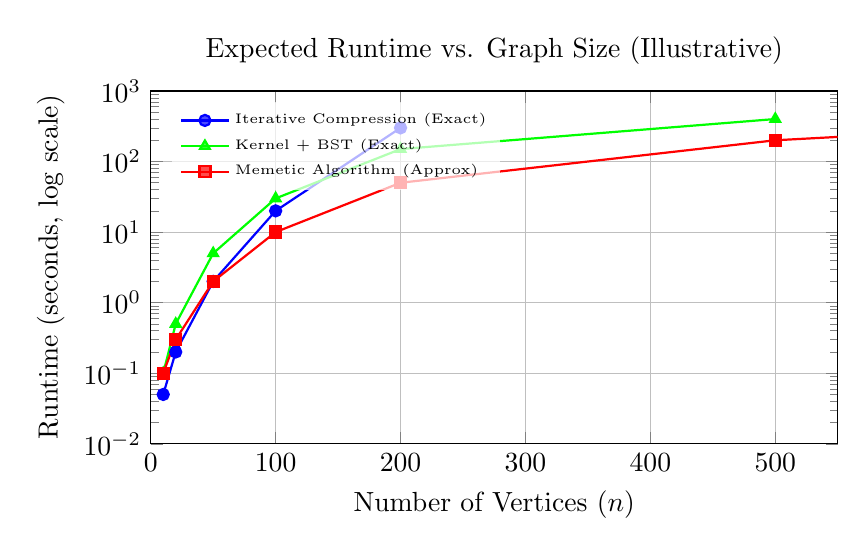
\begin{tikzpicture}
			\begin{axis}[
					title={Expected Runtime vs. Graph Size (Illustrative)},
					xlabel={Number of Vertices ($n$)},
					ylabel={Runtime (seconds, log scale)},
					ymode=log,
					xmin=0, xmax=550,
					ymin=0.01, ymax=1000,
					legend style={font=\tiny, draw=none, fill=white, fill opacity=0.7, text opacity=1, cells={anchor=west}},
					legend style={font=\tiny, draw=none, fill=white, fill opacity=0.7, text opacity=1, cells={anchor=west}},
					legend pos=north west,
					grid=major,
					width=0.85\textwidth,
					height=0.5\textwidth
				]

				\addplot[color=blue,thick,mark=*] coordinates {
						(10,0.05) (20,0.2) (50,2) (100,20) (200,300)
					};
				\addlegendentry{Iterative Compression (Exact)}

				\addplot[color=green,thick,mark=triangle*] coordinates {
						(10,0.1) (20,0.5) (50,5) (100,30) (200,150) (500,400)
					};
				\addlegendentry{Kernel + BST (Exact)}

				\addplot[color=red,thick,mark=square*] coordinates {
						(10,0.1) (20,0.3) (50,2) (100,10) (200,50) (500,200) (1000,600)
					};
				\addlegendentry{Memetic Algorithm (Approx)}

			\end{axis}
		\end{tikzpicture}
		\caption{Hypothetical runtime comparison showing expected scalability trends. Actual results will be empirically determined.}
	\end{figure}
	
	\vspace{0.2cm}
	\footnotesize
	\textbf{Key Observation:} We expect exact algorithms to struggle beyond $n \approx 200$, while GA maintains reasonable performance on large instances.
\end{frame}




\section{Applications}

\begin{frame}{Applications}
	\begin{block}{Overview}
		\begin{itemize}
			\item Survey theoretical and practical applications of \fvs.
			\item Provide domain examples: OS deadlocks, VLSI testing, biology, social networks, finance.
			\item Discuss impact and real-world relevance of solutions.
		\end{itemize}
	\end{block}
\end{frame}




\begin{frame}{Application 1 : Deadlock Detection in Operating Systems}
	\begin{columns}[T]
		\column{0.55\textwidth}
		\textbf{Problem}
		\begin{itemize}
			\item Processes compete for shared resources
			\item Circular waiting leads to deadlock
			\item Goal: resolve deadlock with minimal impact
		\end{itemize}

		\vspace{0.15cm}

		\textbf{Graph Model}
		\begin{itemize}
			\item Vertices represent processes
			\item Directed edges represent wait-for relations
			\item Cycles correspond to deadlocks
		\end{itemize}

		\vspace{0.15cm}

		\textbf{Role of FVS}
		\begin{itemize}
			\item FVS models processes whose removal breaks all cycles
		\end{itemize}

		\column{0.45\textwidth}
		\centering
		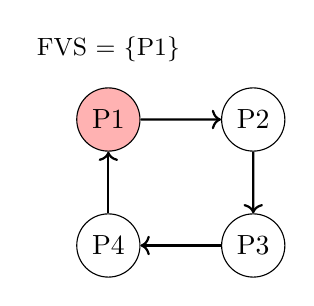
\begin{tikzpicture}[scale=0.80]
			\node[circle,draw,fill=red!30] (P1) at (0,2) {P1};
			\node[circle,draw] (P2) at (2.3,2) {P2};
			\node[circle,draw] (P3) at (2.3,0) {P3};
			\node[circle,draw] (P4) at (0,0) {P4};

			\draw[->,thick] (P1) -- (P2);
			\draw[->,thick] (P2) -- (P3);
			\draw[->,thick] (P3) -- (P4);
			\draw[->,thick] (P4) -- (P1);

			\node[above=0.2cm of P1] {\small FVS = \{P1\}};
		\end{tikzpicture}

		\vspace{0.2cm}
		{\small\textit{Deadlock cycle in a wait-for graph}}
	\end{columns}
\end{frame}



\begin{frame}{Application 2: VLSI Circuit Testing}
	\begin{columns}[T]

		\column{0.6\textwidth}
		\textbf{Challenge}
		\begin{itemize}
			\item Modern chips contain millions of logic gates
			\item Feedback loops make testing computationally hard
			\item Acyclic circuits are testable in linear time
		\end{itemize}

		\vspace{0.1cm}

		\textbf{FVS-Based Solution}
		\begin{itemize}
			\item Model circuit as a graph
			\item Compute a small \fvs\ to break all cycles
			\item Fix FVS gates and test remaining acyclic circuit
			\item Test FVS gates separately
		\end{itemize}

		\vspace{0.1cm}
		\column{0.35\textwidth}
		\hspace{-0.4cm}
		\begin{block}{Example}
			\begin{itemize}
				\item 32-bit ALU circuit
				\item 5,000 gates total
				\item 200 feedback paths
				\item \fvs\ size: 50 gates
			\end{itemize}

			Fixing 50 gates $\Rightarrow$ 4,950 acyclic gates

			\vspace{0.2cm}

			\textbf{Benefits}
			\begin{itemize}
				\item Reduced test time
				\item Lower power consumption
				\item Smaller hardware overhead
			\end{itemize}
		\end{block}
	\end{columns}
\end{frame}



\begin{frame}{Application 3: Gene Regulatory Networks}
	\begin{columns}[T]
		\column{0.5\textwidth}
		\textbf{Biological Motivation}
		\begin{itemize}
			\item Genes regulate each other via feedback loops
			\item Cycles control cell behavior and disease states
		\end{itemize}

		\vspace{0.1cm}

		\textbf{Graph Model}
		\begin{itemize}
			\item Vertices: genes
			\item Edges: regulatory interactions
			\item Cycles: feedback regulation
		\end{itemize}

		\vspace{0.1cm}

		\textbf{Role of FVS}
		\begin{itemize}
			\item Small set of \fvs\ genes controls all feedback : Interpreted as \textbf{master regulators}
			\item Targets for intervention and experiments
		\end{itemize}

		\column{0.4\textwidth}
		\begin{block}{Cancer Study Example}
			\begin{itemize}
				\item Breast cancer regulatory network
				\item 500 genes analyzed
				\item \fvs: 12 key genes
				\item 10 known and 2 novel drug targets
			\end{itemize}
		\end{block}

		\vspace{0.2cm}

		\textbf{Applications}
		\begin{itemize}
			\item Drug target discovery
			\item Gene knockout analysis
			\item Personalized medicine
		\end{itemize}

	\end{columns}
\end{frame}


\begin{frame}{Social and Financial Networks}

	\begin{block}{Social Network Analysis}
		\begin{itemize}
			\item Feedback loops amplify influence and information spread
			\item \fvs\ nodes correspond to key influencers or superspreaders
			\item Targeting \fvs\ improves marketing efficiency
			\item Disrupting \fvs\ reduces misinformation propagation
		\end{itemize}
	\end{block}

	\begin{block}{Financial Systemic Risk}
		\begin{itemize}
			\item Financial institutions form highly interconnected networks
			\item Cycles represent circular dependencies and systemic risk
			\item \fvs\ identifies systemically important institutions
			\item Used for regulation, monitoring, and crisis prevention
		\end{itemize}
	\end{block}
\end{frame}



\begin{frame}{Theoretical Applications}
	\begin{itemize}
		\item \textbf{Complexity Theory}
		      \begin{itemize}
			      \item Used in NP-completeness reductions
			      \item Benchmark problem for cycle-breaking hardness
		      \end{itemize}

		      \vspace{0.2cm}

		\item \textbf{Algorithm Design}
		      \begin{itemize}
			      \item Testbed for FPT(Fixed Parameter Tractable) techniques
			      \item Motivates iterative compression and branching methods
		      \end{itemize}

		      \vspace{0.2cm}

		\item \textbf{Approximation Theory}
		      \begin{itemize}
			      \item Used to study approximation limits
			      \item Reference problem for constant-factor approximations
		      \end{itemize}

		      \vspace{0.2cm}

		\item \textbf{Graph Structure Analysis}
		      \begin{itemize}
			      \item Tool for analyzing treewidth and feedback structure
			      \item Applied in kernelization and graph decompositions
		      \end{itemize}
	\end{itemize}
\end{frame}

% ============================================
% SECTION 7: FUTURE WORK
% ============================================
\section{Potential Research Directions}

\begin{frame}{Potential Research Directions}
	\begin{block}{Overview}
		\begin{itemize}
			\item Highlight open theoretical problems (approximation gap, faster FPT, kernels).
			\item Point out practical directions: ML integration, dynamic and distributed algorithms.

		\end{itemize}
	\end{block}
\end{frame}


\end{document}